\documentclass[fleqn,10pt]{wlscirep}
\usepackage[utf8]{inputenc}
\usepackage[T1]{fontenc}
\renewcommand{\familydefault}{\sfdefault}

\linespread{1.5}

% TITLE PAGE %%%%%%%%%%%%%%%%%%%%%%%%%%%%%%%%%%%%%%%

\title{Lessons on the quality of tuberculosis diagnosis from 2,943 standardized patients in three low- and middle-income countries}

\author[1]{Benjamin Daniels}
\author[1,2]{Ada Kwan}
\author[3]{Madhukar Pai}
\author[1,4]{Jishnu Das}
\affil[1]{Development Research Group, The World Bank, Washington, DC, USA}
\affil[2]{University of California at Berkeley, Berkeley, CA, USA}
\affil[3]{McGill International TB Centre and Department of Epidemiology and Biostatistics, McGill University, Montreal, QC, Canada}
\affil[4]{Center for Policy Research, New Delhi, India}

\begin{abstract}
Standardized patients (SPs) are people who are recruited locally, trained to make identically scripted clinical presentations, deployed incognito to multiple different health care providers, and debriefed using a structured reporting instrument. The use of SPs has increased dramatically as a method for assessing quality of TB care since it was first validated and used for tuberculosis in 2015. This paper summarizes common findings using a combined sample of 2,943 SP-provider interactions involving tuberculosis across various sampling strata in published studies from India, China and Kenya. It then discusses the lessons learned from implementing standardized patients in these diverse settings. First, quality is low: relatively few SPs presenting to a health care provider for the first time were given an appropriate diagnostic test, and most were given unnecessary or inappropriate medication. Second, care takes a wide variety of forms – SPs did not generally receive ``wait and see'' or ``palliative'' care from providers, but they received a medley of care patterns that included broad-spectrum antibiotics as well as contraindicated quinolone antibiotics and steroids. Third, there is a wide range of estimated quality in each observed sampling stratum: more-qualified providers and higher-level facilities performed better than others in all settings, but in every stratum there were both high- and low-quality providers. Finally, providers responded to experimental differences in case presentation that give some clues as to the reasons for these behaviors.
\end{abstract}

\begin{document}

\flushbottom
\maketitle

\thispagestyle{empty}
\newpage

% MAIN TEXT %%%%%%%%%%%%%%%%%%%%%%%%%%%%%%%%%%%%%%%

\section*{Introduction}

Tuberculosis (TB) remains one of the most deadly diseases in the world, having caused an estimated 1.6 million deaths in 2017 with higher mortality than HIV/AIDS.\cite{world2018global} Part of the reason that TB mortality is now estimated to be higher than that from HIV/AIDS is that massive global investment in better diagnosis and anti-retroviral treatment has drastically reduced HIV/AIDS mortality. Additionally, TB is a tenacious disease that is progressively becoming harder and more expensive to cure, with increasing prevalence of strains that display drug resistance to the standard treatment regimen around the world.

Tackling TB requires renewed investments in every step of the care cascade leading patients to successful diagnosis treatment. In South Africa, the TB care cascade shows that just 53\% of suspected cases end up being successfully treated: 5\% are lost at test access, 13\% at diagnosis, 12\% at treatment initiation and 17\% at successful treatment completion.\cite{naidoo2017south} The situation is similar in India.\cite{subbaraman2016tuberculosis} In China, TB prevalence has declined sharply from 215 in 1990 to 108 in 2010, thanks to improved treatment access for those who were already diagnosed,\cite{whochina} but the fraction of TB patients who remain undiagnosed remains high.\cite{sylvia2017tuberculosis}

Recent improvements in treating those who have already been diagnosed with TB reflect better program design, guided by research on treatment adherence and new drugs and regimens.\cite{schnippel2018effect,for2018treatment} Unfortunately, achieving similar gains in timely and accurate detection of individuals with TB in the first place has proven harder. Difficulties in directly measuring the quality of primary care and providers' diagnostic accuracy implies that we do not know how patients presenting with TB symptoms are managed at different stages of the disease. At this point, we cannot answer the question: "In Country X, what do the doctors do when a patient arrives, presenting with 3 weeks of cough, fever and night sweats?" Our relative ignorance about how TB patients are actually managed during this first critical interaction is particularly surprising, as delays at the diagnosis and treatment initiation stage allow patients to remain contagious and continue to spread the disease among their contacts. In fact, several systematic reviews show that TB is often diagnosed after about 2 months of delay, with several visits before diagnosis.\cite{sreeramareddy2014delays,sreeramareddy2009time}

In order to address this gap, researchers have developed and applied the method of standardized patients (SPs) to measure the quality of TB diagnosis and treatment in multiple settings directly. With the SP method, the research team recruits and trains a team of local people to present as patients with the same set of pre-scripted symptoms (in this case, early signs of TB) to a sampled set of health care providers.\cite{das2015use} Health care providers do not know when they are interacting with a standardized patient, and therefore researchers are able to obtain accurate measures of the management that real patients presenting similar symptoms would receive.

Quality of care can be measured in many ways, but many methods observe only imperfect measures. By observing process quality directly, the SP method improves on ``structural'' quality measures which may not predict actual clinical performance, such as the availability of equipment and medicine.\cite{das2007variations} The SP method also has several advantages relative to quality measures based on clinical observation and chart abstraction. Because the underlying condition of the SP is fixed and known by design, the appropriateness of clinical action (or inaction) can be assessed against pre-determined checklists; by contrast, any medical records that do exist may contain incomplete information on patients and recorded diagnoses may be incorrect. Presentation standardization further implies that an individual SP can present the ``same'' case to many providers, allowing valid comparisons across providers and locations. Since the SP presents unannounced to clinics, SP studies avoid ``Hawthorne effects'', whereby providers change their behavior when they know they are being observed.\cite{leonard2006outpatient,das2015use} Finally, training SPs to accurately recall each clinical encounter allows for the use of an extensive, detailed, structured exit questionnaire for each interaction to answer specific research questions.

Following previous large SP studies using asthma and angina cases in India,\cite{das2012urban,das2016quality} our team extended the SP method to evaluate the quality of TB care in a 2015 pilot.\cite{das2015use,heap2019} In our validation study, we showed that the SP method for TB was (a) observationally valid, with low detection rates and high agreement between audio recordings and structured questionnaires; (b) reliable, with key regularities documented in the data; and (c) informative, allowing researchers to understand both the overall quality of care and variation in care across different purposively selected groups of providers. Since the pilot, research groups have used the SP method to study the quality of TB care in full-scale samples across multiple settings in India, China, Kenya, and South Africa. \cite{daniels2017use,kwan2018variations,sylvia2017tuberculosis,das2015use,christian2018measuring}

Here, we summarize global findings using a combined sample of 2,943 SP-provider interactions across those three countries using data from the published studies. We first focus on 1,718 provider-patient interactions with an SP portraying a classic suspected TB case -- the ``Classic'' scenario -- which was used in all these studies, where the SP presented with two weeks of cough to a health care provider for the first time, and with prompting reveals additional symptoms such as fever and night sweats. We then contrast these with findings from 1,225 additional TB presentations in India, which included SPs who report to have already undergone a chest X-ray or laboratory sputum test, and with SPs who presented with classic symptoms of multi-drug resistant TB.

We document the overall quality of care in these settings, both in terms of whether SPs received appropriate care and whether they received unnecessary or harmful medicines. The latter include fluoroquinolone antibiotics and steroids, which can mask TB symptoms from future diagnosis. We then demonstrate the variability in care across settings and types of providers that the SPs visited. Finally, using variations in case presentation from India, we explore the reasons for poor quality as well as potential differences in diagnosis and treatment by SP characteristics.

\section*{Methods}
In each of these primary studies, conducted after ethics approvals in each country, research teams recruited healthy individuals from the local population, who were then extensively trained to present TB cases to health care providers. Every SP was trained for several weeks to portray a single case presentation. The training focused on embedding the medical details of the case within the overall character of the SP in a consistent manner and further ensured that providers would not be able to distinguish the SPs from regular patients during the interactions.

Each study developed SP scripts detailing what information the SP was to give the provider at the beginning of the interaction, typically a short sentence in the local language such as: ``Doctor, I have a cough that is not getting better and some fever too.'' The scripts further specified exact responses to anticipated follow-up history questions from providers, including a scripted personal background, family and socioeconomic situation, and health history details such as smoking and alcohol use. SPs were coached on avoiding unsafe situations and avoiding detection by the providers. The exact details of each study's SP recruitment, provider selection, and fieldwork implementation can be found in the respective primary studies and their online supplements.\cite{daniels2017use,kwan2018variations,sylvia2017tuberculosis} Further general details on the SP method are available in a series of pilot and full-scale studies.\cite{rethans1991method,glassman2000using,das2012urban,satyanarayana2016use,sylvia2014survey} 

Finally, SPs were trained to recall all aspects of the interaction including the questions that the provider asked, the examinations they performed, the tests ordered and any treatment given. These were then recorded in a structured questionnaire shortly after the SP left the providers' clinic. The questionnaire was developed through an extensive consultation process with a technical advisory group composed of local and global TB experts in each country. While SP presentations can vary contextually, all studies used the ``Classic'' presentation that was characterized as ``a case of presumed tuberculosis with 2–3 weeks of cough and fever''. In accordance with national and international guidelines as well as the recommendations of the advisory group, the SP was judged to have been correctly treated if he/she received either a chest X-ray, a sputum AFB test or an Xpert MTB/RIF diagnostic. 

We report on 1,718 Classic TB SP presentations completed between 2015 and 2018 in these three settings. For each study, we investigated the following quality outcomes: the proportion of ``history checklist questions'' completed; whether the provider ordered a chest X-ray, a sputum AFB  or an Xpert MTB/RIF diagnostic; whether any medication was given or prescribed; use of any antibiotics; whether any anti-TB medication was used; and the use of any contraindicated steroids or fluoroquinolone antibiotics. This analysis reports unweighted proportions only, and the results reported here should not be considered to be nationally-representative comparisons for any of the constituent studies.

We present separate estimates of quality of care outcomes for the Classic TB presentation by each study's primary sampling strata. In Kenya, SPs visited both public sector and private sector (for-profit and nonprofit) clinics in Nairobi; private sector providers account for a majority of all providers in the city. In India, all interactions were in the private sector and SPs visited ``informal'' and ``formal'' private sector clinics in urban Patna, and AYUSH and hospital-based private providers in Mumbai. Informal providers in Patna are those without MBBS (allopathic) degree qualifications; such providers account for 42\% of all providers in Patna. AYUSH providers are those with a degree in alternative systems of medicine covering Ayurveda, Yoga, Unani, Siddhi and Homeopathy. In China, SPs visited village, township, and county-level public providers across three provinces (Sichuan, Shaanxi, and Anhui) . Training and expertise in China increases at higher levels of care, moving from the village to the county. The exact details of the sampling strata and the sampling and visitation protocols are available in each study. 

We also present additional results from the studies in urban India, where the team prepared and completed three additional case scenarios with different SPs, resulting in an additional 1,225 SP interactions presenting one of the following:

\begin{itemize}
\item A case of presumed TB in a patient who has had 2–3 weeks of cough and fever. The patient has taken a broad-spectrum antibiotic (amoxicillin) given by another health-care provider for one week with no improvement. The SP also carries an abnormal chest X-ray suggestive of tuberculosis.
\item Chronic cough with an AFB-positive sputum smear report for TB from a public health facility, highly suggestive of TB.
\item Chronic cough, and, if asked, elaborates a history of previous, incomplete treatment for TB, which would raise the suspicion of multi-drug-resistant TB.
\end{itemize}

\noindent These case presentations were each conducted among a statistically comparable subset of the providers who also saw an SP giving the Classic TB presentation. This sampling design allows differences between the actions of the providers to be attributed to the change in case presentation rather than other confounding factors. Therefore, we compare these additional cases separately to the Classic TB case presentation on the same outcome measures.

\section*{Results}

\subsection*{Management of the Classic TB case presentation}

We report three main findings for the Classic case presentation. First, the use of appropriate TB testing varies widely across the study population, ranging from 4\% among informal private clinics in Patna to 90\% in county-level public hospitals in China. As can be seen in \textbf{Figure 1}, testing frequency was substantially higher in higher-level clinics than in lower-level clinics (in China), in formal clinics and hospitals than in informal clinics and Ayush providers (in India), and public clinics than in private clinics (in Kenya). Chest X-rays were the most popular TB test ordered in India and China, in 36\% of interactions; in Nairobi both public and private sector providers preferred sputum smears, in 50\%. At the time of these studies, Xpert MTB/RIF testing was just becoming available and was observed only among Mumbai providers in hospitals (3\%).   

Second, all types of providers (although not all providers) were observed to prescribe some kind of medication to the SP (87\% of interactions), and these were likely to be demonstrably unnecessary or harmful. \textbf{Table 1} highlights three classes of medications which are of special interest for TB treatment: broad-spectrum antibiotics, fluoroquinolone antibiotics and steroids. These medications either have public health implications or are contraindicated in possible TB cases because they may mask symptoms from further diagnosis. We also documented the use of unlabelled, traditional, and homeopathic medicines whose provenance is unknown; the use of such medicines are problematic as they convey no information to the patient. Strikingly, cases where none of these medicines were used are in the minority everywhere. We observe every possible combination of these medications in the data at least once, with providers in every study setting using antibiotics frequently.

Finally, we use adherence to an essential checklist of history questions to examine variation in quality of care within every setting and strata. \textbf{Figure 2} illustrates this variation. While the practices of different groups in each study differ \textit{on average}, there is a broad range of observed provider behavior within each group as well. In no study did any provider type strictly dominate all the others. Instead, these provider type and qualification classifications were weakly associated with provider behavior, and the variations are wide within each. Every strata group contains providers who ask many questions from the checklist; and providers who ask very few. 

\subsection*{Management of other tuberculosis case presentations}
In the India study, SPs also presented three other TB case scenarios with very different backgrounds from the Classic case at a subset of the same providers, allowing direct comparability between management in those cases and in the Classic case. The first panel in \textbf{Figure 3} summarizes TB-related management across all cases for each of the sample strata, highlighting the use of TB testing (chest X-ray, sputum AFB smear, or Xpert MTB/RIF); anti-TB medication; and contraindicated steroids and fluoroquinolone antibiotics.

For all types of providers, the use of TB testing was higher when the SP carried an AFB-positive sputum smear report, even though the SP clearly indicates that he/she does not know what the test implies. This is also true for the case presenting the abnormal chest X-ray in all but one strata. The second panel reports usage of contraindicated steroids and fluoroquinolone antibiotics. The white markers show overall rates of fluoroquinolone usage for each of the three cases; the black markers show the usage of steroids. As in the overall data for the Classic TB case, there are no clear patterns and wide variation in usage across both strata and case presentation.

Finally, since the India study used a relatively larger number of individual SPs in order to accommodate the scale of the study, we investigate the role their individual identities played in their treatment outcomes. \textbf{Figure 4} uses the individual characteristics of the SPs we hired in an ANOVA analysis. We add these characteristics sequentially to a regression model after controlling for the case presentation, study setting and provider type. The first panel shows that SP age, gender, height, weight, and BMI do not significantly contribute to explaining variation in TB testing. In the second panel, we use an individual indicator variable (dummy) for every SP used in both studies to fully test for differences across all specific individuals. Although we cannot rule out the null hypothesis that SP identity indicators are jointly significant -- they seem to have some effect -- we observe that the overall variation in outcomes due to all SP characteristics is (at most) one-fourth the variation explained by case presentation, city, and strata indicators.

\section*{Discussion}
Following our study validating the use of SPs to measure the quality of TB care, researchers have successfully deployed SPs in large provider samples across multiple countries. These studies are tailored to the country context, and therefore differ in their sampling schemes and providers covered; consequently, we have been able to show that the SP methodology can be successfully used for a variety of providers (public, private, formal, informal, AYUSH) in multiple settings.

Three regularities have emerged from these studies. First, appropriate TB testing increases as expected at higher levels of care--formal providers and hospitals in India, and county doctors in China were more likely to appropriately test patients for TB when symptoms warrant. Second, even as appropriate testing increases at higher levels of care, the inappropriate use of medicines does not decline proportionally. In fact, formal providers and hospitals in India, and township clinics in China were just as likely to use antibiotics and quinolones as their less-qualified counterparts. Similarly, care was better in the public sector in Nairobi than the private secrot, but medication use was identical. Third, even though higher levels of care are associated with greater use of appropriate testing, there is always wide variability in quality within every setting and strata. There are always \textit{some} informal providers who did more than \textit{some} formal providers in India; \textit{some} village clinics that did more than \textit{some} township hospitals in China; and \textit{some} private providers that did more than public providers in Nairobi.

One important question these studies raise is whether it is fair to expect health care providers to recommend TB tests on a new patient's very first visit. Cities like Patna and Mumbai in India are polluted and conditions associated with chronic coughs are common. In these situations, it may be appropriate for providers to recommend cough suppressants and move to TB testing if the symptoms do not subside. We are sympathetic to this critique. However, two patterns in the data lead us away from this specific interpretation. First, it does not appear that providers are following a general ``alternate'' protocol where medicines are used for symptomatic relief prior to further testing. Instead, we find widespread use of all types of medicine combinations, including those that can lead to resistance and mask TB symptoms in the future. Second, providers at higher levels of care are always more likely to recommend appropriate treatments. This suggests that even if our benchmarks of appropriate treatment are unrealistic, they remain helpful in ranking different types of providers in a manner that is consistent with their practice setting and qualifications. Rather than limiting analysis to a binary definition of right and wrong, rich SP data can be used to classify providers across a multidimensional quality spectrum, and these classifications can be further refined by using auxiliary information such as the completion of checklist items.

A second question raised by these studies is the reasons for frequent misdiagnosis. One possibility is that providers do not have the knowledge to diagnose patients appropriately. However, studies from India and China were able to directly compare performance with SPs to tests of knowledge on the same conditions and demonstrate a ``know-do gap'' in the data. Providers misdiagnosed SPs at a much higher rate than what tests of knowledge would suggest.

Another possibility is that providers--particularly those in the private sector--deliberately misdiagnose patients to maximize their revenue when patients return. Our data from case variants where the SP provides a positive test result show that even if revenue considerations are part of the explanation they cannot be the \textit{only} reason for frequent misdiagnosis. When SPs carry a positive test result, misdiagnosis declines even if providers take a financial loss from doing so. Since SPs indicate to the provider that they cannot interpret the test result, the providers should not have changed their behavior if their only aim was to maximize their revenues. These results suggest instead that providers face systematic barriers in their attempts to diagnose TB patients that are unrelated to knowledge or financial incentives. What these barriers are requires further research.

A final concern with SP studies is that the individual identity of the SPs could dramatically affect study results, and many studies use only a small number of individual people as SPs. In these studies, SPs were hired from a healthy working population and selected for their ability to accurately and reliably perform a very difficult job in the field. It could be that providers are being systematically misled by the appearance or behavior of these SPs, leading them away from a TB diagnosis. However, as the same SPs were used for all providers, the higher frequency of appropriate treatment among formal providers and at higher levels of care mitigates against this possibility: ``better'' providers were more likely to believe that the SPs actually had TB, it appears. In addition, by using detailed staff information from the large study in India, we are now able to look directly at the correlations between quality of care and data on SP gender, height, weight, BMI and age; and by comparing individual SPs directly. Typically, SP characteristics have little bearing on the quality of the interaction and, though we cannot rule out individualized effects completely, we show that they are small relative to differences across providers and cases and seem to be nothing more than the normal noise that any diverse patient population would entail -- there is, after all, no perfect ``Classic Case''.

With these broad-based results, we believe that SP studies therefore satisfy multiple demanding requirements for the reliable measurement of diagnostic and treatment accuracy for TB. We have made substantial progress in addressing several open questions that have been raised following our initial validation study. Nevertheless, the SP method suffers from several limitations that will need further investigation. Currently, we cannot construct full care cascades for SPs following a misdiagnosis in the first interaction. Suppose the provider asks the SP to return if he/she is not improving -- what happens next? In these studies, SPs simply never went back. We have now carried out a small (unpublished) field pilot to investigate the ability of the SP method to be useful here; the principal difficulty is that a single intial SP presentation can quickly morph into various ``un-standardized'' cases as each SP will likely have received a different treatment in the first instance. Furthermore, we have only partial answers to why misdiagnoses are so frequent, and why providers continue to use a cocktail of antibiotics, steroids and quinolones to treat patients with 2-3 weeks of cough, which may mask TB symptoms, rather than immediately suggesting a TB-sensitive test like an X-ray (if only to rule it out). We suspect that the widespread use of incorrect medicines may be linked to financial incentives and this is a further area to explore, especially given the rapid rise of anti-microbial resistance in countries like India. Indeed, ethnographic and qualitative research now suggests that multiple pressures drive the widespread empirical practices observed, including the use of medications as diagnostic tools, a desire to provide rapid symptom relief to patients, a desire to manage illness costs effectively, uncertainty about the presentation of TB, and uncertainty about the accuracy of available TB tests.\cite{mcdowell2016treatment}

\section*{Ethical Approval}

Each of the studies from which data was utilized here obtained ethical approval from the relevant institutional review boards. This study exclusively relied on data obtained from those studies and therefore has not obtained separate ethical approval.

\section*{Competing Interests}

None of the authors have any competing interests to disclose.

\section*{Acknowledgements}

The findings, interpretations, and conclusions expressed here are those of the authors and do not necessarily represent the views of the World Bank, its executive directors, or the governments they represent.

\section*{Data Availability Statement}

Individual de-identified interaction data, including data dictionaries, will be available. All variables needed to re-create the results reported in this article will be included, as will the code required to reproduce these results. Data will be available indefinitely upon publication to anyone who wishes to access the data for any purpose. The data and code can be accessed at \url{https://github.com/qutubproject/jclintb2019}.

% BACKMATTER %%%%%%%%%%%%%%%%%%%%%%%%%%%%%%%%%%%%%%%

\newpage

\bibliography{sample}

\newpage

\section*{Table 1: Use of unnecessary and contraindicated medications for the Classic TB case}

\begin{figure}[h]
\centering
\includegraphics[width=1\textwidth]{meds.png}
\end{figure}

\noindent\textit{Note:} Medications from each interaction were ex-post coded by name to correspond to ATC code classifications, the WHO system for categorizing medications according to their purpose and action. This figure reports the whole number of SP interactions in which each combination of the following medicine classes were observed to have been given to the patient, and the corresponding proportion of interactions in that sampling stratum. The categories are: broad-spectrum antibiotics (other than fluoroquinolones), defined as ATC codes beginning with J01 but not J01M; fluoroquinolone antibiotics, defined as ATC codes beginning with J01M; steroids, defined as ATC codes beginning with H02, R01, or R03; and unlabelled medications, for which the field team was unable to identify generic ingredients (including homeopathic, traditional, and herbal medications, but excluding vitamin and mineral preparations). Percentages may not add to 100\% due to rounding.

\newpage

\section*{Figure 1: Classic TB case management by study and strata}

\begin{figure}[h]
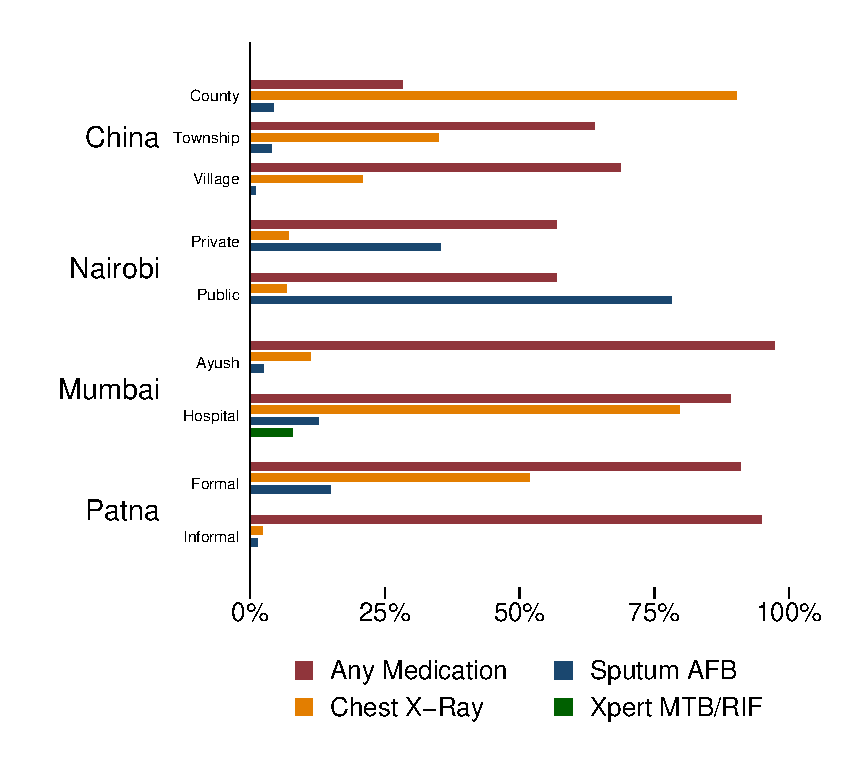
\includegraphics[width=1\textwidth]{f1.eps}
\end{figure}

\noindent\textit{Note:} This figure reports the overall proportion of SPs presenting the Classic TB case in each study who received each of the indicated management decisions by the provider. Number of observations: China County (21), Township (207), Village (71); Nairobi Private (28), Public (14); Mumbai Ayush (499), Hospital (305); Patna Formal (389), Informal (184). Xpert MTB/RIF usage was observed only in Mumbai Hospital sample. AFB: Acid-Fast Bacillus; MTB/RIF: Mycobacterium Tuberculosis/Rifampicin.

\newpage

\section*{Figure 2: History checklist completion for the Classic TB case: variation by study and strata}

\begin{figure}[h]
\centering
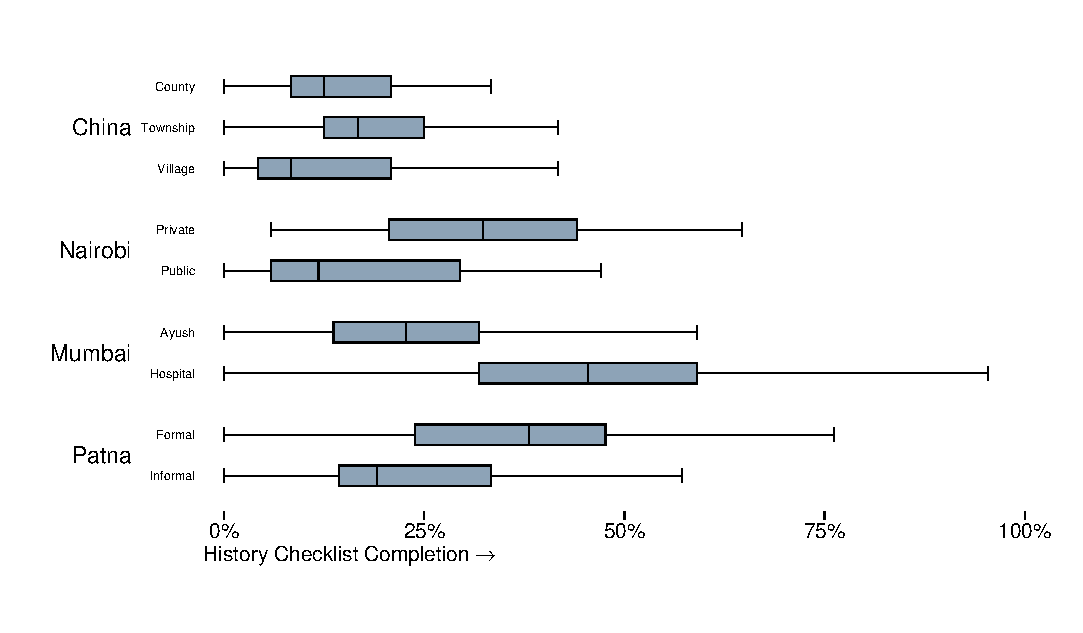
\includegraphics[width=1\textwidth]{f3.eps}
\end{figure}

\noindent\textit{Note:} Using the context-specific measure of history checklist items, this figure illustrates the range of item completion within each study and sampling strata. Number of observations: China County (21), Township (207), Village (71); Nairobi Private (28), Public (14); Mumbai Ayush (499), Hospital (305); Patna Formal (389), Informal (184). History checklist questions: Duration of Cough, Sputum, Past TB, Family TB, Blood in Sputum, Cough Throughout Day, Fever, Fever Type, Family or Family with Similar Symptoms, Chest Pain, Loss of Appetite, Lost Weight, Wheezing, Difficulty Breathing, Smoking, Alcohol History, Taken Medicines for Illness, Diabetes, HIV/AIDS, Age, TB Suspicion, MDR-TB Suspicion, High blood pressure or hypertension, Weakness, Night Sweats.

\newpage

\section*{Figure 3: TB-related testing, anti-TB medication, and contraindicated medication use by case presentation in urban India for all case presentations}

\begin{figure}[h]
\centering
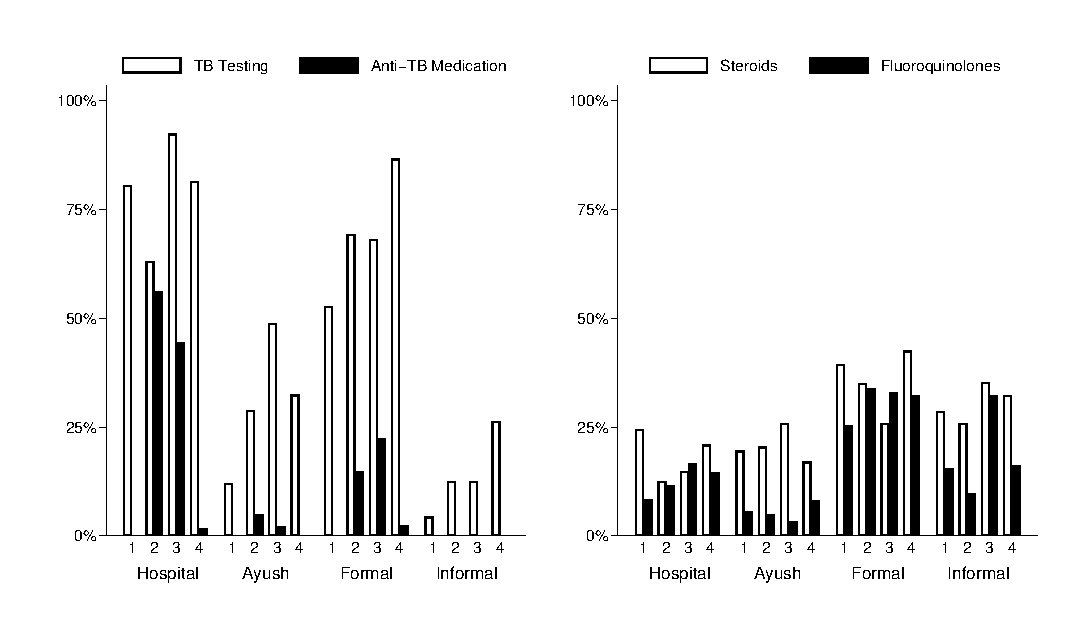
\includegraphics[width=1\textwidth]{f4.eps}
\end{figure}

\noindent\textit{Note:} This figure reports the usage of laboratory testing, anti-TB medication, fluoroquinolone antibiotics, and steroids across each study strata for four case presentations. These were the Classic TB presentation (A); the X-ray presentation (B); the sputum report presentation (C); and the MDR presentation (D). Hospital and Ayush providers were in Mumbai; Formal and Informal providers in Patna.

Number of observations: Mumbai Ayush Classic (499), X-ray (125), Sputum (125), MDR (247); Mumbai Hospital Classic (305), X-ray (122), Sputum (79), MDR (81); Patna Formal Classic (389), X-ray (98), Sputum (110), MDR (120); Patna Informal Classic (184), X-ray (40), Sputum (40), MDR (38). Medications from each interaction were ex-post coded by name to correspond to ATC code classifications. This figure reports the proportion of SP interactions in which each of the following medicine classes were observed to have been given to the patient: fluoroquinolone antibiotics, defined as ATC codes beginning with J01M; and steroids, defined as ATC codes beginning with H02, R01, or R03.

\newpage

\section*{Figure 4: ANOVA analysis of explained variation of TB testing to individual SP characteristics for all case presentations}

\begin{figure}[h]
\centering
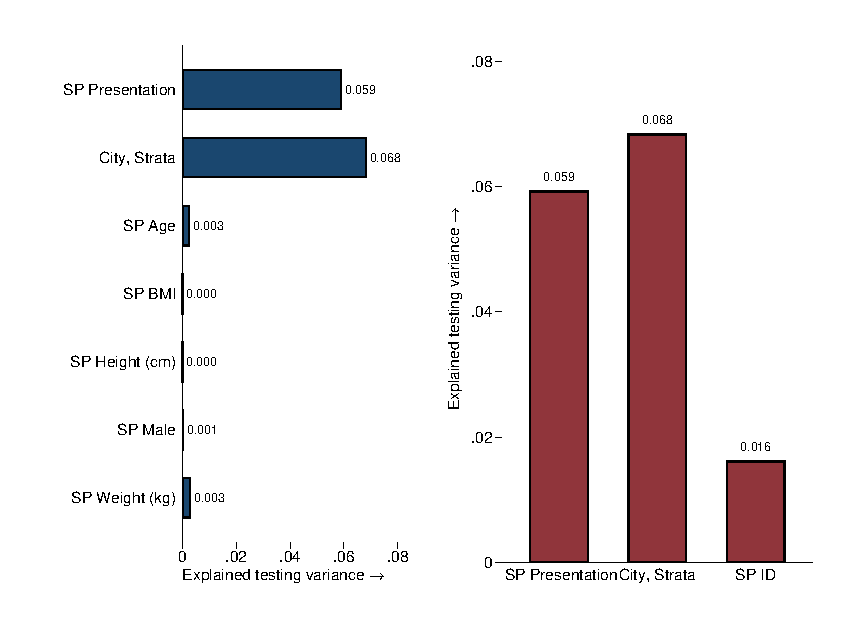
\includegraphics[width=1\textwidth]{f5.eps}
\end{figure}

\noindent\textit{Note:} This figure reports the sequential-ANOVA contribution of SP characteristics to the explained variance of receiving any of the following: a chest X-ray, a sputum AFB smear, or an Xpert MTB/RIF test. The binary outcome is first regressed on SP presentation and study location and strata, and in the first panel, individual characteristics are sequentially added and the improvement in explained sum of squares reported. In the second panel, the entire set of individual SP identity indicators is added to the regression and its overall contribution to explained variation in TB-testing outcomes is reported. AFB: Acid-Fast Bacillus; MTB/RIF: Mycobacterium Tuberculosis/Rifampicin.

\end{document}